\pagestyle{empty}
\setstretch{1.2}
\begin{center}
\textbf{\large{ОТВЕТЫ, УКАЗАНИЯ, РЕШЕНИЯ}}
\end{center}
\begin{minipage}{0.45\textwidth}
\begin{center}
\so{К статье}

"\so{Рассказ о кванте}"

\so{(стр. 6-15)}
\end{center}
\textbf{1.} $9,8 \cdot 10^{-7}$ \textit{дж/см}$^2$


\textbf{2.} $2,3 \cdot 10^{-12}$ эрг $\sim 1,5$ электрон-вольта. Максимум числа квантов: $1,7 \cdot 10^{-12}$ эрг $\sim 1$ электрон-вольт.


\textbf{3.} $4.4 \cdot 10^{12}$ квантов в оном кубическом сантиметре.

\textbf{4.}Энергия кванта: $9,6$ килоэлектрон-вольта, энергия электрона: $0,1$ килоэлектрон-вольта

\begin{center}
"\so{К статье Цепные дроби}"
\so{(стр. 16-26)}
\end{center}
\par\textbf{1.} $\lambda = 5215,5$.
\par\textbf{2.} $\left[0; 1, 2, 3, 4, 5\right]$.
\par\textbf{3.} $\frac{5777}{1875}$

\begin{itemize}
\item[a)] $\left[1; 1212\cdots\right]$,
\item[b)] $\left[2; 444\cdots\right]$,
\item[c)] $\left[2; 2424\cdots\right]$.
\end{itemize}

\textbf{5.} б) $\frac{\sqrt{ab(ab - 4)} - ab}{2a}*)$.

\begin{center}
\so{К статье}

"\so{Что такое функция}"

\so{(стр. 27-36)}
\end{center}

 \textbf{1.}Естественная облась определения: а) $ x\ne 0;$ б) $x \le -1; x \ge 1$

 \textbf{4.} а) $9$; б) $8$; в) $6$.

\textbf{5.} а) $9$; б) $8$; в) $9$; г) $0$.

\textbf{6.} $10^7 \cdot 4^7$

\textbf{8.} $n^m$

\textbf{12.} Обратимы $f_1$ и $f_3$.

\textbf{13} и \textbf{14.} Отображение совпадает с обратным к нему.

\textbf{16.} а)1680; б)9240; в) $18 150 = 3^9 - 3\cdot 2^9 + 3$.

\textbf{18.} $A_n^m = n (n - 1)\ldots (n- m + 1)$, если $m \le n$; $A_n^m = 0$, если $m > n$.

\textbf{20.} $\frac{28!}{(7!)^4}$

\noindent\rule{2cm}{0.4pt}

$*)$ Это -- положительный корень уравнения
\begin{equation}
  x = \cfrac{1}{a 
          + \cfrac{1}{b + x } }
\end{equation}
\textbf{62}
\end{minipage}
\hfill
\begin{minipage}{0.45\textwidth}
\begin{center}
\so{К статье}

"\so{Сухое трение}"

\so{(стр. 37-43)}
\end{center}
\textbf{1.} Разложим силы трения, ействующие на передние колеса автомобиля, на две составляющие: $F_1$, лежащие в плоскости колес, и $F_2$, перпендикулярные колесам (см. рисунок). Силы $F_1$ заставляют колеса вращаться, а силы $F_2$ поворачивают автомобиль.
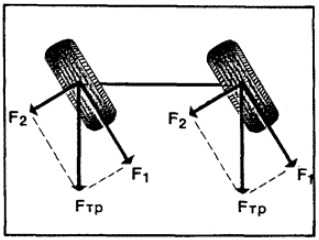
\includegraphics[scale=1]{lab62.jpg}

\textbf{2.} Если центр тяжести палки не находится посередине межу пальцами, но давление палки на кольцо различно. Различны и силы тяготения, действующие на палку со стороны пальцев. Палка смещается в ту сторону, где трение меньше.

\textbf{3.} Пока брусок не скользит по плоскости, сила трения равна по величине проекции веса бруска на наклонную плоскость $F_{TP} = P\sin \alpha$. Брусок начинает скользить, когда сила трения достигает максимальной величины трения покоя $F_{TP} = k N = k P\cos \alpha$. При этом выполняется условие $k P\cos \alpha = P\sin \alpha$. Поэтому соскальзывание бруска начинается при угле наклона плоскости к горизонту $\alpha = \arctan k$. После этого сила трения будет равна $F_{TP} = k N = k P\cos \alpha$.

Угол $\alpha = \arctan k$, при котором брусок начинает скользить, называют углом трения. Он имеет еще и другой геометрический смысл: если к бруску, лежащему на горизонтальной плоскости, приложить силу, составляющую с вертикалью угол меньший, чем угол трения, то брусок нельзя сдвинуть с места, сколь велика ни была бы приложенна сила. Доказать это можно так. Посадим наблюдателя на наклонную плоскость, на которой лежит бру-
\end{minipage}
\begin{spacing}{1.5}
Например, про отображение
$$
x \to |x|
$$
можно сказать, что оно является отображением $R$ в $R$, но нельзя сказать, что это "отображение $R$ на $R$".

С чисто логической точки зрения наиболее простым является случай, когда область определения функции конечна. Ясно, что функция, область определения которой состоит из $n$ элементов, не может принимать более $n$ различных значений. Таким образом, функции, определенные на конечных множествах, осуществляют отображения конечных множеств на конечные множества. Таки отображения являются одним из предметов изучения важной части математики - \textit{комбинаторики} (см. задачи 8, 11, 18, 19)

\so{Пример 4}. Рассмотрим функции, область определения которых есть множество
$$
M = \{A, B\}
$$
из двух букв $A$ и $B$ и значения которых принадлежат тому же множеству, т.е. отображения множества $M$ в себя.

Таких функций существует всего \so{четыре}. Зададим их табличным способом:
\end{spacing}
\begin{center}
\begin{tabular}{ | l | l | l | l |l |}
\hline
x& $f_1 (x)$ & $f_2 (x)$ & $f_3 (x)$ & $f_4 (x)$ \\ \hline
A & A & B & A & B \\
B & A & B & B & A \\
\hline
\end{tabular}
\end{center}